\documentclass[conference]{IEEEtran}
\IEEEoverridecommandlockouts
\usepackage{cite}
\usepackage{amsmath,amssymb,amsfonts}
\usepackage{algorithmic}
\usepackage{graphicx}
\usepackage{textcomp}
\usepackage{xcolor}
\usepackage{booktabs}
\usepackage{tabularx}
\usepackage{multirow}
\usepackage{url}
\usepackage{tikz}
\usetikzlibrary{shapes.geometric, arrows.meta, positioning, calc}

\renewcommand{\topfraction}{0.95}
\renewcommand{\bottomfraction}{0.95}
\renewcommand{\textfraction}{0.05}
\renewcommand{\floatpagefraction}{0.85}
\renewcommand{\dbltopfraction}{0.95}
\renewcommand{\dblfloatpagefraction}{0.85}

\def\BibTeX{{\rm B\kern-.05em{\sc i\kern-.025em b}\kern-.08em
    T\kern-.1667em\lower.7ex\hbox{E}\kern-.125emX}}

\begin{document}

\title{A Leakage-Safe Audit of Network Telemetry for\\Manufacturing Efficiency in a Synthetic\\Smart-Factory Benchmark}

\author{\IEEEauthorblockN{Atharva Gangurde}
\IEEEauthorblockA{B.Tech. Candidate in Artificial Intelligence \& Data Science\\
MVP Samaj's Karmaveer Adv. Baburao Ganpatrao Thakare College of Engineering\\
Nashik, Maharashtra, India\\
Email: atharvagangurde12345@gmail.com}
}

\nocite{haque2025urllc, ibrahim2025urllc, paudyal2025gnb, alves2021beyond, tgpp22104, kapoor2023leakage, kaufman2012leakage, lopez2018advances, cena2021redundancy, zunino2024adaptive, ferrari2011wireless, vitturi2019industrial, popovski20185g, breiman2001random, ke2017lightgbm, chen2016xgboost, seabold2010statsmodels, dickey1979distribution, granger1969investigating, benjamini1995controlling, andrews1993tests, hansen2000sample, pedregosa2011scikit, lundberg2017unified, rousseeuw1987silhouettes, davies1979cluster, calinski1974dendrite, gangurde2026repository}
\maketitle

\begin{abstract}
Smart manufacturing research increasingly considers low-latency, highly reliable communication as an enabler of coordinated cyber-physical production. Yet predictive studies based on industrial telemetry can be undermined by temporal leakage, target contamination, and benchmark data that do not encode physical network--process coupling. This paper presents a leakage-aware statistical audit of a smart-factory telemetry benchmark containing 100,000 records from 50 machines over approximately 68.4 days. We examine marginal distributions, pairwise correlations, target-label construction, temporal precedence, candidate latency breakpoints, unsupervised clusters, and predictive performance under chronological and machine-grouped evaluation. One-sample Kolmogorov--Smirnov diagnostics, whose uniform bounds were estimated from the observed data, do not reject any marginal distribution after Bonferroni correction; these results are treated as diagnostics rather than proof of a joint independent-uniform generating process. None of the 36 pairwise Pearson correlations remains significant after family-wise correction. The efficiency label is almost exactly reproduced by a rule using error rate and production speed, and the class distribution is highly imbalanced (77.825\% Low and 2.986\% High). In Active mode, a data-selected latency breakpoint of 20.69\,ms appears significant under a naive asymptotic test ($p = 0.0378$) but is not supported by the implemented supremum-$F$ permutation analysis ($p = 0.1640$, FDR $q = 0.5100$). Across the reported leakage-aware model configurations, ROC-AUC ranges from 0.4738 to 0.5073. The benchmark therefore provides no convincing evidence that network telemetry alone predicts the composite efficiency label. The findings emphasize that dataset provenance, target construction, dependence-aware inference, and realistic validation must be established before drawing operational conclusions about network quality of service.
\end{abstract}

\begin{IEEEkeywords}
Industrial Internet of Things, smart manufacturing, network telemetry, data leakage, statistical audit, changepoint detection, machine learning, synthetic data.
\end{IEEEkeywords}

\section{Introduction}
\label{sec:intro}

\subsection{Networked Manufacturing and the 6G Context}
The integration of telecommunications and industrial automation is central to Industry 4.0 and the emerging Industry 5.0 vision. Research on sixth-generation (6G) wireless systems considers very low latency, tight jitter bounds, and high communication reliability for mission-critical cyber-physical production systems. Such capabilities are relevant to coordinated robotic workcells, distributed programmable logic controllers (PLCs), edge-based computer vision, and automated guided vehicle (AGV) routing~\cite{haque2025urllc, ibrahim2025urllc, paudyal2025gnb, alves2021beyond}. These values should be understood as targets associated with specific future systems and use cases, rather than universal performance guarantees for deployed 6G networks.

The 3rd Generation Partnership Project (3GPP) Technical Specification TS 22.104 describes communication-service requirements for cyber-physical control applications in vertical domains, including scenarios with stringent latency and message-transfer constraints~\cite{tgpp22104}. In smart factories, network telemetry such as latency and packet loss may be analyzed alongside operational technology (OT) signals such as temperature, vibration, power consumption, and production speed. Whether these telemetry streams contain useful predictive information, however, is an empirical question that depends on the data-generating process and evaluation design.

\subsection{Leakage and Benchmark Validity}
Predictive studies can report optimistic or misleading performance when train and test sets contain temporally adjacent observations, overlapping machine histories, or features that directly encode the target. Such leakage can permit a model to reproduce a labeling rule rather than learn a relationship that generalizes to a future time period or an unseen machine~\cite{kapoor2023leakage, kaufman2012leakage, lopez2018advances}. Class imbalance can compound the problem: a model may appear accurate while failing to identify a rare but operationally important state.

A related concern is benchmark validity. Synthetic data can be useful for testing software and analytical procedures, but independently generated features may omit the feedback loops expected in a physical manufacturing system. Statistical associations, clusters, or thresholds found in such data should not automatically be interpreted as evidence of real industrial regimes.

\subsection{Research Questions}
This study evaluates the evidential value of network telemetry using five research questions (RQs), summarized in Table~\ref{tab:rq}.

\begin{table}[t]
\caption{Research Questions Addressed in This Study}
\label{tab:rq}
\centering
\footnotesize
\begin{tabularx}{\columnwidth}{@{}l X@{}}
\toprule
\textbf{ID} & \textbf{Core investigation} \\
\midrule
\textbf{RQ1} & Are marginal feature distributions and pairwise linear associations consistent with the benchmark's apparent synthetic structure? \\
\textbf{RQ2} & Do the analyzed latency series exhibit evidence of unit-root behavior, and does past latency improve prediction of production speed in the tested Granger models? \\
\textbf{RQ3} & Are data-selected latency breakpoints robust after accounting for the threshold search? \\
\textbf{RQ4} & Do network-telemetry clusters provide evidence of distinct operational regimes, rather than geometric partitions? \\
\textbf{RQ5} & How well does network telemetry predict efficiency under chronological and machine-grouped validation when direct target components are excluded? \\
\bottomrule
\end{tabularx}
\end{table}

\subsection{Contributions}
The paper makes four contributions. First, it combines marginal-distribution diagnostics, pairwise correlation testing, and an audit of the benchmark's efficiency-label rule. Second, it compares naive breakpoint significance with a supremum-$F$ permutation analysis and documents the sensitivity of results to data-driven threshold selection. Third, it evaluates clustering and predictive models using temporal and machine-grouped splits while excluding contemporaneous ingredients of the target from the feature matrix. Fourth, it describes a reproducible analysis pipeline and makes its code and report artifacts available in the associated project repository~\cite{gangurde2026repository}.

\section{Related Work}
\label{sec:related_work}

Research in industrial wireless communication has examined redundancy, path diversity, and reliable message delivery for mobile industrial applications. Cena \textit{et al.} studied packet replication and diversity in industrial wireless networks~\cite{cena2021redundancy}; Zunino \textit{et al.} examined adaptive seamless redundancy for MQTT communication~\cite{zunino2024adaptive}. Work on wireless model-based predictive control has shown that network delay can affect control-loop behavior when transport effects are not adequately compensated~\cite{ferrari2011wireless}. Surveys describe the transition from industrial Ethernet and IIoT toward 5G and related communication technologies~\cite{vitturi2019industrial}, while communication-theoretic studies characterize trade-offs among throughput, delay, reliability, and network slicing~\cite{popovski20185g}.

\begin{table*}[t]
\caption{Representative Related Work in Industrial Communication and Predictive Validation}
\label{tab:related_work}
\centering
\scriptsize
\setlength{\tabcolsep}{3pt}
\begin{tabularx}{\textwidth}{@{}l >{\raggedright\arraybackslash}p{4.2cm} >{\raggedright\arraybackslash}p{2.6cm} >{\raggedright\arraybackslash}p{2.2cm} X@{}}
\toprule
\textbf{Reference} & \textbf{Study focus} & \textbf{Domain} & \textbf{Evidence source} & \textbf{Relevance to this paper} \\
\midrule
Cena \textit{et al.}~\cite{cena2021redundancy} & Redundancy and diversity in wireless networks for mobile industrial applications & Industrial wireless & Factory testbed & Shows how communication design can bound delay and improve reliability in a physical setting. \\
Zunino \textit{et al.}~\cite{zunino2024adaptive} & Adaptive seamless redundancy for highly dependable MQTT communication & IIoT messaging QoS & Emulation/testbed logs & Studies adaptive path selection for critical industrial telemetry. \\
Ferrari \textit{et al.}~\cite{ferrari2011wireless} & Wireless model-based predictive networked control & Networked control & Closed-loop testbed & Motivates measuring network effects in relation to control behavior. \\
Vitturi \textit{et al.}~\cite{vitturi2019industrial} & Industrial communication systems and their future challenges & Industrial communication & Survey and standards & Places industrial latency and reliability requirements in context. \\
Popovski \textit{et al.}~\cite{popovski20185g} & Communication-theoretic view of 5G network slicing & Wireless slicing & Analytical/simulation & Describes delay, throughput, and reliability trade-offs. \\
Kapoor and Narayanan~\cite{kapoor2023leakage} & Leakage and reproducibility in machine-learning-based science & ML methodology & Literature review & Explains why leakage-aware evaluation is needed before performance claims are trusted. \\
\textbf{This study} & \textbf{Distribution, label, temporal, breakpoint, clustering, and prediction audit} & \textbf{Smart-factory telemetry} & \textbf{Synthetic benchmark} & \textbf{Tests whether the available benchmark supports the intended predictive or operational interpretation.} \\
\bottomrule
\end{tabularx}
\end{table*}

In applied machine learning, leakage is a recognized source of invalid generalization claims. Kapoor and Narayanan surveyed reproducibility concerns in machine-learning-based science~\cite{kapoor2023leakage}, while Kaufman \textit{et al.} formalized leakage mechanisms and avoidance strategies~\cite{kaufman2012leakage}. Random Forest and gradient-boosted trees are widely used for tabular prediction~\cite{breiman2001random, ke2017lightgbm, chen2016xgboost}; however, model capacity cannot compensate for a benchmark whose features lack the physical relationships the study intends to measure. The present work focuses on this evidence gap by auditing the benchmark before interpreting predictive scores as evidence of network impact.

\section{Methodology and Dataset Audit}
\label{sec:methodology}

\subsection{Pipeline Overview}
The pipeline comprises four linked modules: (1) distribution and label audit; (2) temporal and breakpoint analysis; (3) unsupervised network-telemetry profiling; and (4) leakage-aware prediction. Fig.~\ref{fig:architecture} summarizes the data flow. The analyses are diagnostic: the study does not treat statistical association alone as proof of a causal network effect.

\begin{figure*}[t]
\centering
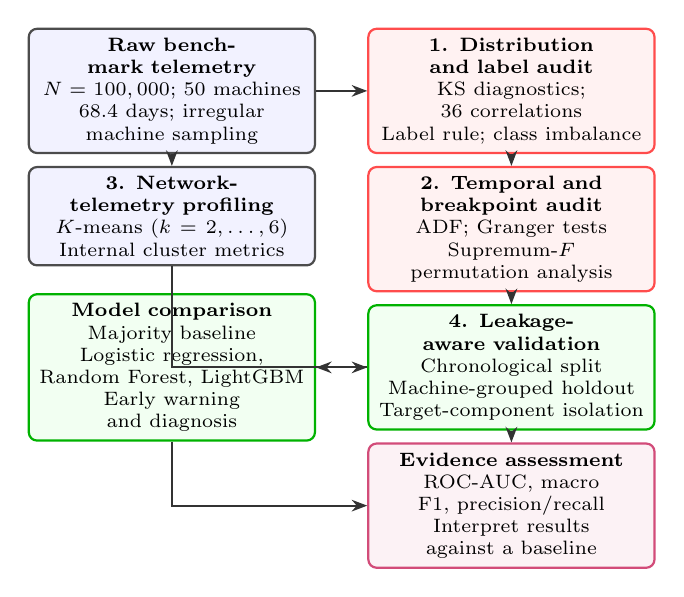
\begin{tikzpicture}[
    node distance=0.15cm and 0.65cm,
    block/.style={rectangle, draw=black!70, fill=blue!5, thick, rounded corners=3pt, text width=3.4cm, minimum height=0.55cm, align=center, font=\scriptsize},
    audit/.style={rectangle, draw=red!70, fill=red!5, thick, rounded corners=3pt, text width=3.4cm, minimum height=0.55cm, align=center, font=\scriptsize},
    model/.style={rectangle, draw=green!70!black, fill=green!5, thick, rounded corners=3pt, text width=3.4cm, minimum height=0.55cm, align=center, font=\scriptsize},
    eval/.style={rectangle, draw=purple!70, fill=purple!5, thick, rounded corners=3pt, text width=3.4cm, minimum height=0.55cm, align=center, font=\scriptsize},
    arrow/.style={-{Stealth[scale=0.85]}, thick, draw=black!80}
]

% Nodes
\node (raw) [block] {\textbf{Raw benchmark telemetry}\\$N=100,000$; 50 machines\\68.4 days; irregular\\machine sampling};
\node (audit) [audit, right=of raw] {\textbf{1. Distribution\\and label audit}\\KS diagnostics; 36 correlations\\Label rule; class imbalance};
\node (temp) [audit, below=of audit] {\textbf{2. Temporal and\\breakpoint audit}\\ADF; Granger tests\\Supremum-$F$\\permutation analysis};
\node (clust) [block, below=of raw] {\textbf{3. Network-\\telemetry profiling}\\$K$-means ($k = 2, \dots, 6$)\\Internal cluster metrics};
\node (split) [model, below=of temp] {\textbf{4. Leakage-aware validation}\\Chronological split\\Machine-grouped holdout\\Target-component isolation};
\node (train) [model, left=of split] {\textbf{Model comparison}\\Majority baseline\\Logistic regression,\\Random Forest, LightGBM\\Early warning and diagnosis};
\node (out) [eval, below=of split] {\textbf{Evidence assessment}\\ROC-AUC, macro\\F1, precision/recall\\Interpret results\\against a baseline};

% Paths
\draw [arrow] (raw) -- (audit);
\draw [arrow] (audit) -- (temp);
\draw [arrow] (raw) -- (clust);
\draw [arrow] (temp) -- (split);
\draw [arrow] (clust) |- (split);
\draw [arrow] (split) -- (train);
\draw [arrow] (train) |- (out);
\draw [arrow] (split) -- (out);

\end{tikzpicture}
\caption{Leakage-aware audit pipeline for the smart-factory telemetry benchmark.}
\label{fig:architecture}
\end{figure*}

\subsection{Dataset and Provenance}
The case study uses the dataset identified in the project materials as \textit{Thales Group Manufacturing Telemetry} and made available through the project repository. The file contains 100,000 records associated with 50 machine identifiers across a stated time span from 2025-01-01 00:00:00 to 2025-03-10 10:39:00 (approximately 68.4 days). The benchmark includes timestamp, machine identifier, operating mode (Active, Idle, or Maintenance), network latency, packet loss, production speed, error rate, defect rate, temperature, vibration, power consumption, and a maintenance score. The report describes irregular per-machine sampling, with a median inter-sample interval of approximately 34 minutes and an interquartile range of 15--68 minutes.

The available materials do not provide evidence that the observations were collected from a physical production line. Accordingly, results are interpreted as findings about this benchmark, which is described as synthetic in the project documentation, rather than as direct measurements of a deployed 5G/6G network or an operating factory.

\subsection{Marginal Distributions and Pairwise Correlations (RQ1)}
For each of nine numeric variables, the original analysis compares the empirical cumulative distribution function (ECDF) with a uniform cumulative distribution over the observed minimum and maximum. The KS statistic is
\begin{equation}
D_N = \sup_{x \in [a, b]} |F_N(x) - F_U(x)|,
\label{eq:ks}
\end{equation}
where $F_N$ is the ECDF and $F_U(x) = (x - a)/(b - a)$. Because $a$ and $b$ are estimated from the observed sample, the conventional one-sample KS reference distribution does not directly provide a fully calibrated test of this composite null. The reported values are therefore retained as exploratory diagnostics; a parameter-estimation-aware test or a suitable simulation-based null should be used for confirmatory inference.

The analysis also calculates the Pearson correlation coefficient for all $\binom{9}{2} = 36$ pairs and applies the Bonferroni correction:
\begin{equation}
p_{\text{adj}} = \min(1, 36 p_{\text{raw}}).
\label{eq:bonferroni}
\end{equation}
This procedure tests pairwise linear association. Failure to reject these pairwise hypotheses does not establish mutual or statistical independence among all variables.

\subsection{Efficiency-Label Audit and Class Imbalance}
The target variable, \textit{Operational Efficiency}, has three classes: $\mathcal{Y} \in \{\text{Low}, \text{Medium}, \text{High}\}$. The label rule inferred from the benchmark is
\begin{equation}
\mathcal{Y} = 
\begin{cases}
\text{Low}, & E > 5.0 \;\lor\; P \le 200, \\
\text{High}, & P > 400 \;\land\; E \le 2.0, \\
\text{Medium}, & \text{otherwise},
\end{cases}
\label{eq:label_rule}
\end{equation}
where $E$ is Error Rate (\%) and $P$ is Production Speed (units/hour). The inferred rule agrees with the supplied labels for 99.998\% of the records; the two mismatched records should be inspected in the preprocessing and label-generation code before the rule is regarded as exact.

If one assumes independent uniform distributions $E \sim \mathcal{U}(0, 15)$ and $P \sim \mathcal{U}(50, 500)$, the rule implies the following reference class probabilities:
\begin{equation}
\begin{aligned}
\Pr(\text{Low}) &= 1 - \frac{1}{3}\cdot\frac{2}{3} = \frac{7}{9} \approx 77.78\%, \\
\Pr(\text{High}) &= \frac{2}{9}\cdot\frac{2}{15} = \frac{4}{135} \approx 2.96\%, \\
\Pr(\text{Medium}) &= 1 - \frac{7}{9} - \frac{4}{135} = \frac{26}{135} \approx 19.26\%.
\end{aligned}
\label{eq:probs}
\end{equation}
These are theoretical values under the stated independence and uniformity assumptions, not proof that the joint distribution follows those assumptions. The empirical class counts are 77,825 Low (77.825\%), 19,189 Medium (19.189\%), and 2,986 High (2.986\%). The Low-to-High ratio is approximately $26.06 : 1$, making class-aware metrics essential.

\subsection{Temporal Diagnostics and Granger Tests (RQ2)}
The Augmented Dickey--Fuller (ADF) test is used to assess the unit-root null for the indexed latency and production-speed series~\cite{seabold2010statsmodels, dickey1979distribution}:
\begin{equation}
\Delta Y_t = \alpha + \beta t + \gamma Y_{t-1} + \sum_{j=1}^p \delta_j \Delta Y_{t-j} + \varepsilon_t.
\label{eq:adf}
\end{equation}
Rejecting the unit-root null is evidence against a unit root under the test specification; it is not by itself a complete demonstration of weak stationarity. This caveat is important because per-machine observations are irregularly spaced and pooled row order is not equivalent to a regular physical-time grid.

Granger-causality tests evaluate whether lagged network latency provides additional predictive information for production speed after accounting for lagged production speed~\cite{granger1969investigating}. For row lags $k \in \{1, 2, 3\}$, the fitted model is
\begin{equation}
P_t = c + \sum_{i=1}^k a_i P_{t-i} + \sum_{i=1}^k b_i L_{t-i} + u_t,
\label{eq:granger}
\end{equation}
with $H_0: b_1 = \dots = b_k = 0$. The report evaluates 450 machine--mode--lag configurations and applies the Benjamini--Hochberg false-discovery-rate (FDR) procedure at $q = 0.05$~\cite{benjamini1995controlling}. Because the lags represent rows rather than fixed elapsed-time intervals, these tests do not estimate a uniform 1-, 2-, or 3-step delay in minutes.

\subsection{Data-Selected Breakpoints (RQ3)}
The segmented regression is
\begin{equation}
P_t = \beta_0 + \beta_1 L_t + \beta_2 (L_t - \tau)_+ + \varepsilon_t,
\label{eq:segmented}
\end{equation}
where $(x)_+ = \max(x, 0)$. Candidate breakpoints are scanned over 81 quantiles between the 10th and 90th percentiles of latency, and the candidate maximizing a Chow-type $F$ statistic is selected. Since the breakpoint is chosen from the data, the resulting maximum statistic does not generally follow the ordinary fixed-breakpoint $F$ reference distribution~\cite{andrews1993tests, hansen2000sample}.

The original analysis uses a vectorized supremum-$F$ Monte Carlo permutation procedure with $B = 2,000$ draws and seed 42. For each draw, it permutes the response vector under the implemented null, recomputes the maximum statistic over the candidate grid, and estimates the exceedance probability as
\begin{equation}
p_{\text{perm}} = \frac{1}{B} \sum_{b=1}^B \mathbf{1}_{\left\{\sup_\tau F^{(b)}(\tau) \ge \sup_\tau F_{\text{obs}}(\tau)\right\}}.
\label{eq:perm_p}
\end{equation}
This procedure accounts for the threshold search in its permutation reference distribution. However, unrestricted response permutation does not preserve within-machine serial dependence; the resulting $p$-values should therefore be interpreted conditionally on the exchangeability assumption used by the implementation. A confirmatory analysis should use dependence-preserving permutations or a null model that explicitly represents machine and temporal structure. The original pooled analysis additionally reports a machine-block bootstrap with 1,000 resamples for breakpoint uncertainty.

\subsection{Unsupervised Profiling (RQ4)}
$K$-means is evaluated for $k = 2, \dots, 6$ on standardized network telemetry. The reported criteria are inertia, silhouette score~\cite{rousseeuw1987silhouettes}, Davies--Bouldin index~\cite{davies1979cluster}, and Calinski--Harabasz index~\cite{calinski1974dendrite}. Internal clustering metrics describe geometric compactness and separation; in the absence of physical labels or a validated generative reference, they do not establish that a cluster corresponds to a distinct operational state.

\subsection{Leakage-Aware Predictive Modeling (RQ5)}
The classification task predicts the three-level efficiency target using scikit-learn and LightGBM~\cite{ke2017lightgbm, pedregosa2011scikit}. To avoid direct target contamination, contemporaneous Error Rate and Production Speed---the inputs to the inferred rule in Eq.~(\ref{eq:label_rule})---are excluded from the predictive feature matrices. The archived experiments report 32 engineered predictors drawn from operational measurements, network latency and packet loss, their row lags, and rolling summaries. The exact feature manifest should be taken from the project code when reproducing the models.

The model comparison includes a majority-class dummy baseline, logistic regression (L2 regularization, $C = 1$, balanced class weights, 1,000 maximum iterations and standardization), Random Forest (200 trees, maximum depth 12, minimum split size 5, balanced class weights), and LightGBM (200 boosting iterations, learning rate 0.05, maximum depth 6, 31 leaves and balanced class weights).

Four experiment configurations are reported: (A) early warning at a physical-time horizon of approximately $30 \pm 10$ minutes ($N = 23,587$); (B) an early-warning sensitivity analysis using a one-row shift ($N = 99,950$); (C) contemporaneous diagnosis with direct target ingredients excluded; and (D) a 30-minute-horizon test on held-out Machines 41--50 after training on Machines 1--40 ($N = 20,016$). Evaluation includes an 80/20 chronological split and a machine-grouped holdout. ROC-AUC confidence intervals are based on 1,000 bootstrap resamples of the test set. SHAP is used for descriptive feature attribution~\cite{lundberg2017unified}.

\section{Empirical Results}
\label{sec:results}

\subsection{Distribution and Correlation Audit (RQ1)}
Table~\ref{tab:ks_uniformity} reports the marginal uniformity diagnostics for the nine numeric features. Production Speed has the smallest raw $p$-value (0.0216), but its reported Bonferroni-adjusted value is 0.1947. None of the nine adjusted tests is significant at $\alpha = 0.05$. Because the bounds were estimated from the same data, this finding should be read as absence of a rejection in the reported diagnostic, not confirmation of a uniform generating process.

\begin{table}[t]
\caption{KS Diagnostics Against Uniform Marginals ($N = 100,000$)}
\label{tab:ks_uniformity}
\centering
\footnotesize
\setlength{\tabcolsep}{3pt}
\begin{tabular}{@{}lcccc@{}}
\toprule
\textbf{Variable} & \textbf{Bounds} & \textbf{$D$} & \textbf{Raw $p$} & \textbf{Adj. $p$} \\
\midrule
Latency (ms) & $[1, 50]$ & 0.003059 & 0.3061 & 1.0000 \\
Packet loss (\%) & $[0, 5]$ & 0.003540 & 0.1627 & 1.0000 \\
Production speed (u/h) & $[50, 499.997]$ & 0.004756 & 0.0216 & 0.1947 \\
Error rate (\%) & $[0, 15]$ & 0.002063 & 0.7873 & 1.0000 \\
Defect rate (\%) & $[0, 10]$ & 0.002680 & 0.4683 & 1.0000 \\
Temperature ($^{\circ}\text{C}$) & $[30, 89.999]$ & 0.001985 & 0.8248 & 1.0000 \\
Vibration (Hz) & $[0.1, 5]$ & 0.001902 & 0.8617 & 1.0000 \\
Power (kW) & $[1.5, 10]$ & 0.002114 & 0.7622 & 1.0000 \\
Maintenance score & $[0.000, 1.000]$ & 0.002850 & 0.3903 & 1.0000 \\
\bottomrule
\end{tabular}
\vspace{0.5ex}
{\raggedright \scriptsize Note: The bounds are sample-estimated; reported $p$-values are retained from the original diagnostic and should not be read as parameter-estimation-aware confirmatory tests.\par}
\end{table}

\begin{table}[t]
\caption{Granger Tests: Latency to Production Speed (450 Configurations)}
\label{tab:granger_summary}
\centering
\footnotesize
\setlength{\tabcolsep}{3.5pt}
\begin{tabular}{@{}lcccc@{}}
\toprule
\textbf{Mode} & \textbf{Tests} & \textbf{Raw $p < .05$} & \textbf{FDR $q < .05$} & \textbf{Significant} \\
\midrule
Active & 150 & 7 (4.7\%) & 0 & No \\
Idle & 150 & 9 (6.0\%) & 0 & No \\
Maintenance & 150 & 7 (4.7\%) & 0 & No \\
\midrule
\textbf{Total} & \textbf{450} & \textbf{23 (5.1\%)} & \textbf{0} & \textbf{0/450} \\
\bottomrule
\end{tabular}
\end{table}

Across the 36 Pearson tests, coefficients lie between approximately $-0.0071$ and $+0.0075$. The largest reported absolute value is between Vibration and Network Latency ($r = 0.007546$, raw $p \approx 0.0170$); after Bonferroni adjustment, $p_{\text{adj}} = 0.6127$. Thus, the analysis finds no pairwise linear association that survives family-wise correction. This result does not rule out nonlinear dependence or dependence involving more than two variables.

\subsection{Temporal Diagnostics and Granger Tests (RQ2)}
The reported ADF statistics are $-14.49$ for latency and $-14.36$ for production speed, with $p < 0.001$ in each case. These results reject the unit-root null for the indexed series under the fitted ADF specifications; because the observations are irregular and include multiple machines, they should not be generalized into a blanket statement of stationarity for each physical process.

Of the 450 tested configurations, 23 have unadjusted $p < 0.05$ (5.1\%), and none remains significant after Benjamini--Hochberg correction. Under the tested model specifications and row-lag definitions, the analysis finds no evidence that past latency adds predictive information for production speed after accounting for the included lags of production speed. This is not proof that network delay has no physical effect in other systems or at other time scales.

\subsection{Breakpoint Analysis (RQ3)}
The active-mode scan selects $\hat{\tau} = 20.69$\,ms. The naive asymptotic test yields $F = 4.3127$ and $p = 0.0378$, whereas the reported supremum-$F$ permutation test yields $p_{\text{perm}} = 0.1640$ and FDR $q = 0.5100$. The candidate threshold is therefore exploratory under the reported procedure, rather than a statistically confirmed operating limit. Table~\ref{tab:breakpoint_results} summarizes all data slices.

\begin{table}[t]
\caption{Breakpoint Results for Latency Versus Production Speed}
\label{tab:breakpoint_results}
\centering
\footnotesize
\setlength{\tabcolsep}{3pt}
\begin{tabular}{@{}lccccc@{}}
\toprule
\textbf{Slice} & $\hat{\tau}$ \textbf{(ms)} & \textbf{Sup-$F$} & \textbf{Naive $p$} & \textbf{Perm. $p$} & \textbf{FDR $q$} \\
\midrule
Pooled & 41.22 & 1.0532 & 0.3048 & 0.7530 & 0.7530 \\
Active & 20.69 & 4.3127 & 0.0378 & 0.1640 & 0.5100 \\
Idle & 27.55 & 1.2800 & 0.2579 & 0.6890 & 0.7530 \\
Maintenance & 25.50 & 3.2382 & 0.0720 & 0.2550 & 0.5100 \\
\bottomrule
\end{tabular}
\end{table}

\begin{figure}[t]
\centering
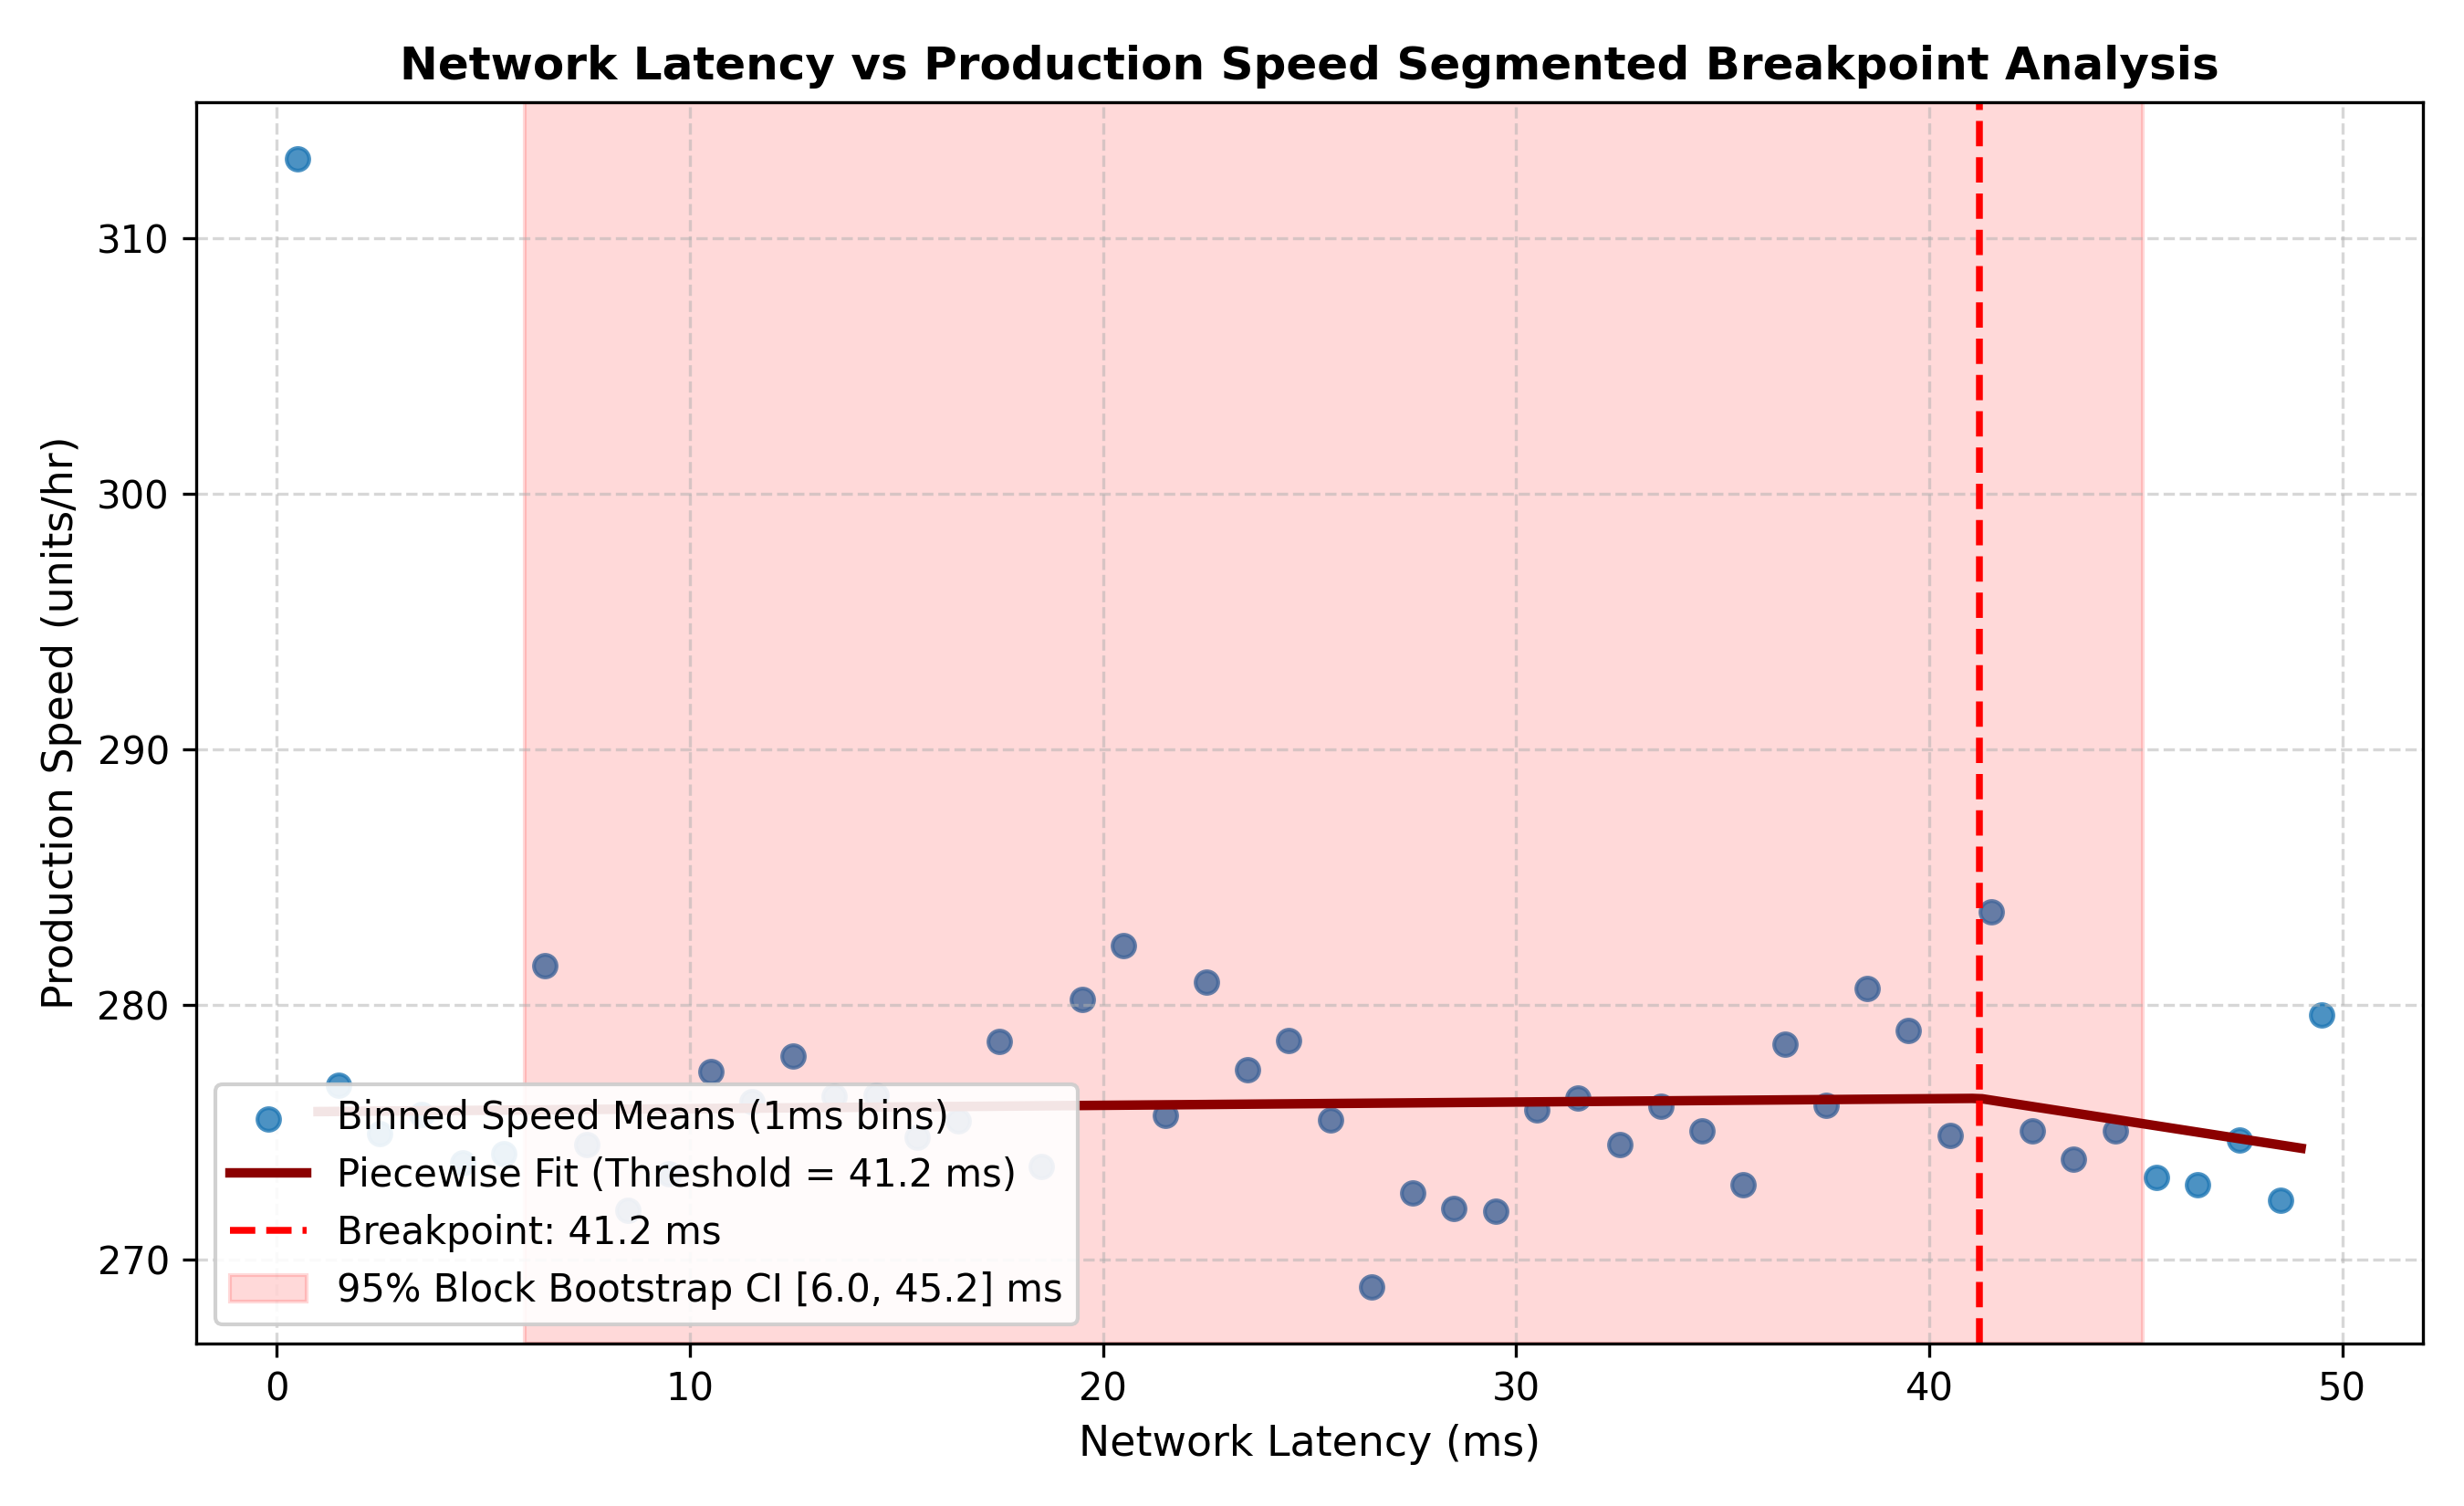
\includegraphics[width=0.68\columnwidth]{figures/latency_breakpoint_segmented_fit.png}
\caption{Segmented fit for pooled latency and production speed. The selected breakpoint is 41.22 ms, but the permutation p-value is 0.7530 and the reported 95\% block-bootstrap interval is wide ([6.0, 45.2] ms). The plot is descriptive and does not establish an operational threshold.}
\label{fig:breakpoint_fit}
\end{figure}

In the implemented permutation experiment, the naive test rejects at nominal $\alpha = 0.05$ in 409 of 2,000 realizations (20.45\%). This demonstrates substantial size distortion in that experiment when the maximum statistic is compared with a fixed-breakpoint asymptotic reference. The precise false-positive rate depends on the permutation null and its dependence assumptions; unrestricted permutation may be inappropriate when serial and machine-level dependence remains. The pooled estimate $\hat{\tau} = 41.22$\,ms has a broad reported 95\% machine-block bootstrap interval of $[6.0, 45.2]$\,ms, further limiting its operational interpretability.

\subsection{Unsupervised Network Profiling (RQ4)}
Table~\ref{tab:clustering_metrics} summarizes K-means metrics for standardized network telemetry. The $k = 4$ solution has the highest reported silhouette score (0.4063) and the lowest Davies--Bouldin index (0.7690) among the tested candidates. These modest internal scores identify a useful geometric partition for describing the data, but without physical state labels or comparison with a suitable null distribution they do not establish four distinct QoS or manufacturing regimes.

\begin{table}[t]
\caption{K-Means Evaluation on Standardized Network Telemetry}
\label{tab:clustering_metrics}
\centering
\footnotesize
\setlength{\tabcolsep}{3.5pt}
\begin{tabular}{@{}ccccc@{}}
\toprule
$k$ & \textbf{Inertia} & \textbf{Silhouette}\textsuperscript{\dag} & \textbf{DB} & \textbf{CH} \\
\midrule
2 & 125,071 & 0.3548 & 1.1871 & 59,910 \\
3 & 79,315 & 0.3764 & 0.8687 & 76,078 \\
\textbf{4} & \textbf{50,230} & \textbf{0.4063} & \textbf{0.7690} & \textbf{99,386} \\
5 & 42,314 & 0.3908 & 0.8367 & 93,161 \\
6 & 35,980 & 0.3745 & 0.8422 & 91,169 \\
\bottomrule
\end{tabular}
\vspace{0.5ex}
{\raggedright \scriptsize \textsuperscript{\dag}Silhouette was calculated on a seeded subsample of 15,000 observations; other indices were calculated on all 100,000 records, as reported in the project artifacts. DB = Davies--Bouldin; CH = Calinski--Harabasz.\par}
\end{table}

\begin{figure}[t]
\centering
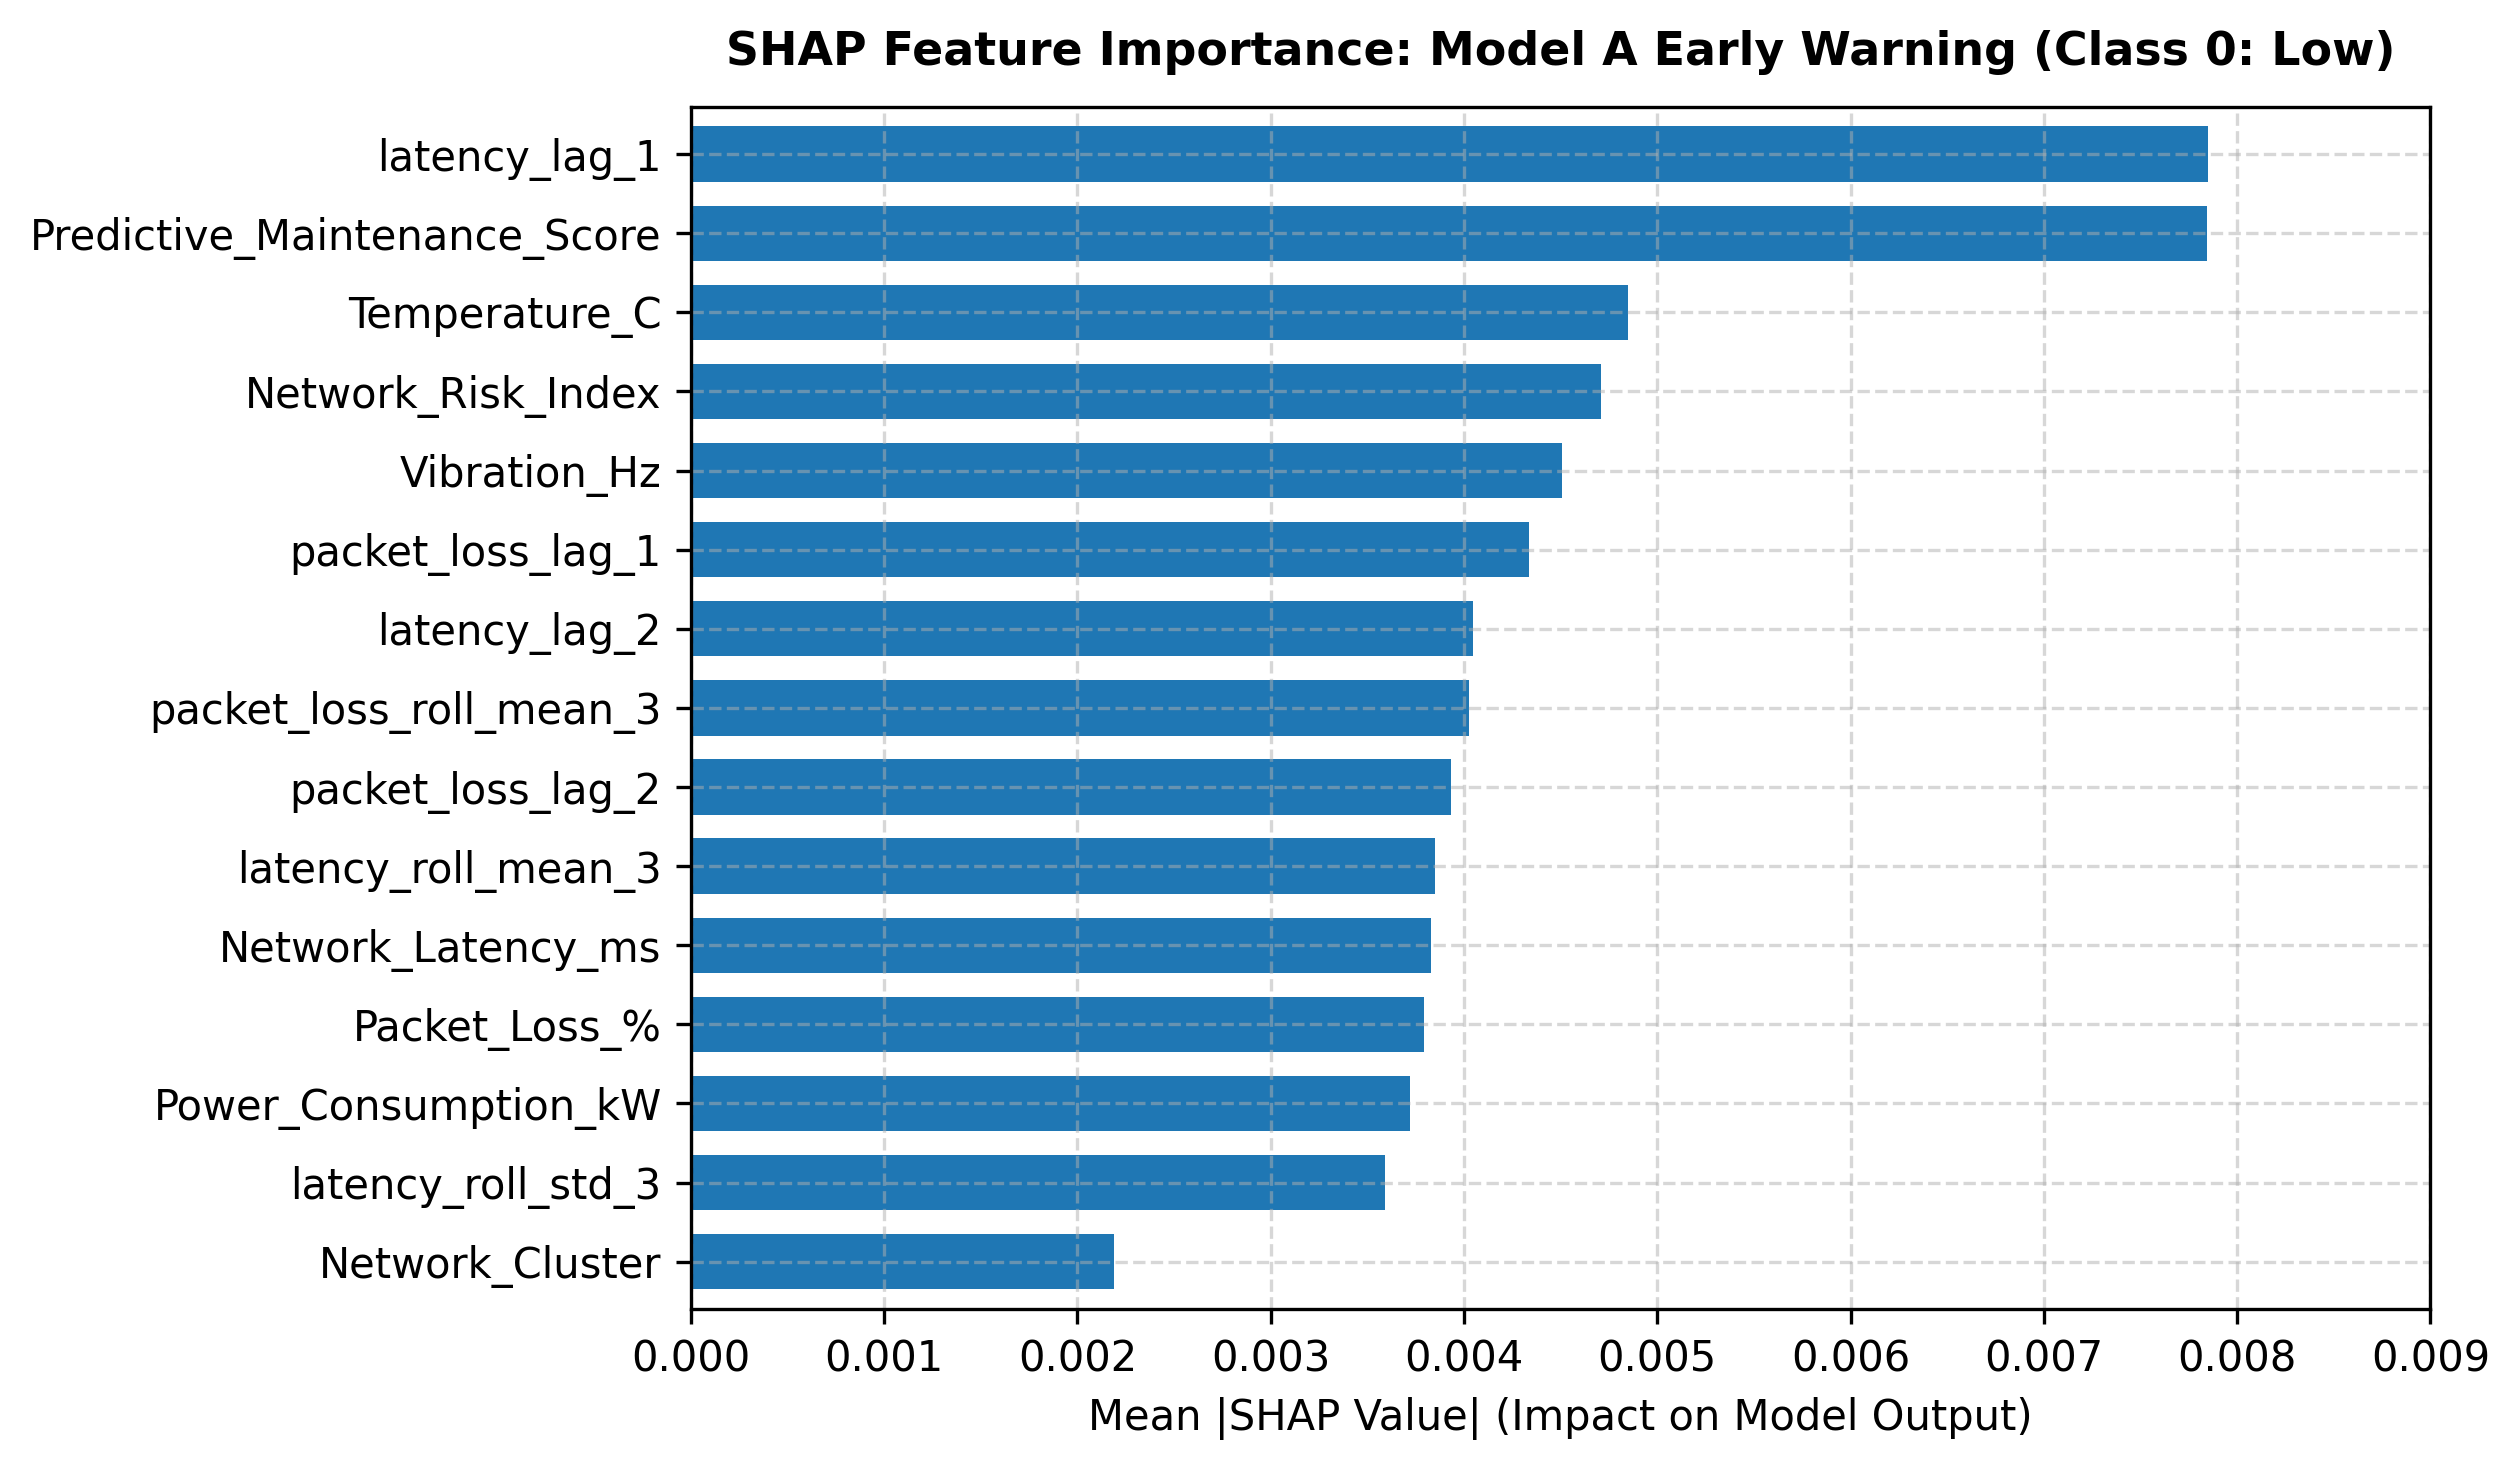
\includegraphics[width=0.60\columnwidth]{figures/shap_summary_model_a.png}
\caption{Mean absolute SHAP values for Model A (early warning, 30-minute horizon) as reported in the project artifact. The largest values are below 0.008. Feature rankings in a near-chance model are descriptive and should not be interpreted as evidence of operational importance.}
\label{fig:shap_model_a}
\end{figure}

\subsection{Predictive Model Performance (RQ5)}
Table~\ref{tab:model_ladder} reports the model scores retained from the original experimental run. ROC-AUC values range from 0.4738 to 0.5073. Most reported 95\% intervals include 0.5; the LightGBM unseen-machine interval is below 0.5. No configuration demonstrates useful discrimination above the random-ranking reference, and the relatively high accuracy of some models must be interpreted alongside the majority baseline and the minority-class metrics.

The Random Forest model in the 30-minute configuration has macro F1 of 0.3368, but High-efficiency recall is only 3.05\%. The comparison between seen-machine and unseen-machine Random Forest results yields macro F1 values of 0.3368 and 0.3275, respectively, while both ROC-AUC intervals include 0.5. These results do not support a claim of meaningful predictive generalization from the available network and sensor features. Because the target is largely determined by production speed and error rate, excluding these contemporaneous components is important; at the same time, the label construction itself limits the extent to which the classification exercise can establish a physical network effect.

\begin{table*}[t]
\caption{Predictive Performance Across Temporal and Machine-Grouped Evaluations}
\label{tab:model_ladder}
\centering
\footnotesize
\setlength{\tabcolsep}{3pt}
\begin{tabularx}{\textwidth}{@{}l l c c c c c c X@{}}
\toprule
\textbf{Configuration} & \textbf{Model} & \textbf{Acc.} & \textbf{Macro F1} & \textbf{Wtd. F1} & \textbf{ROC-AUC [95\% CI]} & \textbf{High-P} & \textbf{High-R} & \textbf{Interpretation} \\
\midrule
\multirow{4}{*}{\textbf{\shortstack[l]{Model A,\\30-min horizon}}} 
 & Dummy majority & 0.7842 & 0.2930 & 0.6894 & 0.5000 [0.5000, 0.5000] & 0.0000 & 0.0000 & Majority-class reference \\
 & Logistic regression & 0.2791 & 0.2321 & 0.3554 & 0.5029 [0.4828, 0.5253] & 0.0302 & 0.4656 & Below majority accuracy \\
 & Random Forest & 0.6730 & 0.3368 & 0.6622 & 0.5068 [0.4856, 0.5296] & 0.0404 & 0.0305 & Near chance \\
 & LightGBM & 0.4313 & 0.2966 & 0.5014 & 0.5073 [0.4863, 0.5283] & 0.0295 & 0.2061 & Near chance \\
\midrule
\multirow{2}{*}{\textbf{\shortstack[l]{Model A,\\one-row shift}}} 
 & Random Forest & 0.5284 & 0.3126 & 0.5742 & 0.4949 [0.4851, 0.5048] & 0.0291 & 0.1117 & Near chance \\
 & LightGBM & 0.3725 & 0.2707 & 0.4470 & 0.4988 [0.4891, 0.5089] & 0.0315 & 0.2709 & Near chance \\
\midrule
\multirow{2}{*}{\textbf{\shortstack[l]{Model B,\\diagnosis}}} 
 & Random Forest & 0.5569 & 0.3246 & 0.5947 & 0.5016 [0.4916, 0.5114] & 0.0240 & 0.0590 & Near chance \\
 & LightGBM & 0.3789 & 0.2733 & 0.4545 & 0.4994 [0.4895, 0.5078] & 0.0300 & 0.2574 & Near chance \\
\midrule
\multirow{2}{*}{\textbf{\shortstack[l]{Unseen machines,\\30-min horizon}}} 
 & Random Forest & 0.7024 & 0.3275 & 0.6717 & 0.4896 [0.4675, 0.5134] & 0.0141 & 0.0078 & No evidence of useful discrimination \\
 & LightGBM & 0.4435 & 0.2889 & 0.5108 & 0.4738 [0.4539, 0.4948] & 0.0215 & 0.1328 & Below chance in this test split \\
\bottomrule
\end{tabularx}
\vspace{0.5ex}
{\raggedright \scriptsize Note: High denotes the minority High-efficiency class (2.986\% prevalence). The unseen-machine configuration trains on Machines 1--40 and tests on Machines 41--50 ($N = 20,016$). The reported 95\% ROC-AUC intervals use 1,000 bootstrap resamples of the test set.\par}
\end{table*}

\section{Discussion}
\label{sec:discussion}

\subsection{Answers to the Research Questions}
\noindent\textbf{RQ1: Distribution.} None of the nine reported marginal KS diagnostics is significant after correction, and no Pearson correlation survives Bonferroni correction. Since the distributional bounds are data-estimated and correlation tests detect only pairwise linear dependence, these results are consistent with weakly coupled synthetic features but do not prove independent uniform generation.

\noindent\textbf{RQ2: Temporal precedence.} The ADF tests reject the unit-root null in the indexed series. No Granger configuration remains significant after FDR adjustment. The evidence is limited to the row-lag model and series construction used in the report; irregular sampling and machine pooling constrain interpretation.

\noindent\textbf{RQ3: Breakpoints.} The Active-mode threshold of 20.69\,ms is significant only under the naive fixed-breakpoint reference. The supremum-$F$ permutation result is not significant under the implemented null, so the breakpoint should not be presented as a validated operational guardrail.

\noindent\textbf{RQ4: Clusters.} The four-cluster solution optimizes two reported internal criteria among $k = 2, \dots, 6$, but these metrics alone cannot establish discrete physical operating regimes.

\noindent\textbf{RQ5: Prediction.} ROC-AUC remains close to 0.5 across the tested configurations, and recall for the rare High class is poor in the principal Random Forest run. The benchmark does not supply convincing evidence that the available network telemetry predicts the composite efficiency label.

\subsection{Implications for Breakpoint Studies}
Selecting a breakpoint by maximizing a statistic over candidate values changes the null distribution of the selected statistic. Applying a fixed-breakpoint asymptotic reference after this search can overstate significance. In the reported permutation experiment, the naive procedure's nominal rejection rate is 20.45\%. A stronger confirmatory design should preserve the relevant machine-level and temporal dependence, report the complete candidate-search procedure, and assess threshold stability across machines and time periods. Sample splitting or methods designed for unknown change points provide additional safeguards~\cite{andrews1993tests, hansen2000sample}.

\subsection{Interpreting Clusters and Feature Importance}
Clustering algorithms partition a feature space even when no physical regimes exist. Inertia and internal separation indices are useful exploratory measures but require a baseline or external validation before clusters are interpreted as QoS classes. Likewise, SHAP ranks model-attributed contributions for the fitted predictor; when out-of-sample discrimination is near chance, those rankings should not be reported as evidence that a feature is physically important.

\subsection{Threats to Validity and Limitations}
Several limitations constrain the conclusions. First, project materials characterize the data as synthetic, and no physical testbed provenance was available to establish real network--process feedback. Second, the KS bounds were estimated from the same sample, so the tabulated $p$-values require a more appropriate calibration for confirmatory goodness-of-fit inference. Third, unrestricted permutation may break temporal and machine-level dependence, while the Granger analysis uses row lags on irregularly spaced observations. Fourth, two records differ from the inferred label rule, and the exact feature manifest should be checked against the preprocessing code. Fifth, the 2,000-draw permutation run and 1,000-resample bootstrap give finite-resolution estimates, and the code should be rerun under a dependence-aware resampling design before the breakpoint analysis is used for an operational decision.

These limitations do not imply that URLLC is unimportant for manufacturing. They mean that this benchmark, in its analyzed form, cannot establish a causal or operational relationship between network quality of service and production efficiency. In physical systems, the impact of latency depends on application timing, control architecture, traffic patterns, redundancy, and failure handling; standards requirements are scenario-specific rather than a single universal threshold~\cite{tgpp22104, vitturi2019industrial}.

\section{Conclusion and Future Work}
\label{sec:conclusion}
This paper presented a leakage-aware audit of a smart-factory telemetry benchmark. The reported marginal-distribution diagnostics and pairwise correlations reveal no corrected statistical evidence of non-uniformity or linear association, while the inferred efficiency rule exposes strong target construction and class-imbalance issues. The Active-mode breakpoint of 20.69\,ms is not supported by the reported supremum-$F$ permutation result, and the supervised models achieve near-chance ROC-AUC under the evaluated temporal and machine-grouped splits. The appropriate conclusion is not that network quality of service has no effect on manufacturing, but that the analyzed benchmark does not provide adequate evidence to quantify such an effect.

Future work should (1) document data provenance and the exact target/feature-generation logic; (2) use goodness-of-fit tests calibrated for estimated parameters; (3) preserve machine-level and temporal dependence in breakpoint inference; (4) align irregular telemetry on a defensible physical-time basis; and (5) validate the pipeline on physical or hardware-in-the-loop industrial testbeds with measured network conditions and production outcomes. The analysis code and supporting artifacts are available at \url{https://github.com/Atharva110409/smart-factory-6g-network}.

\section*{Acknowledgment}
The author acknowledges institutional laboratory support.

\IEEEtriggeratref{21}
\bibliographystyle{IEEEtran}
\bibliography{references}

\end{document}
